\documentclass[a4paper,11pt,fleqn]{article}
\usepackage[utf8x]{inputenc}
\usepackage{ucs}
\usepackage[T2A,OT4]{fontenc}
\usepackage[a4paper,top=2.5cm,bottom=2.5cm,left=2.5cm,right=2.5cm]{geometry}
\usepackage[MeX]{polski}
\usepackage{titling}

%\usepackage{bold-extra}

\usepackage{amssymb}
\usepackage{amsmath}
%\usepackage{amsthm}
%\usepackage{gensymb}

%\usepackage{wrapfig}
\usepackage{graphicx}
%\usepackage{lipsum}
%\usepackage{epstopdf}
\usepackage{caption}
%\usepackage{subcaption}
%\usepackage{adjustbox}
%\usepackage{dcolumn}
%\newcolumntype{d}[1]{D{,}{,}{#1}}


\usepackage{xcolor}
%\colorlet{zaglowek}{blue!10}
\usepackage{indentfirst}
\usepackage{fancyhdr}
\usepackage{lastpage}
%\setlength{\headheight}{13.6pt}
\usepackage{listings}
%\usepackage{slashbox}

\author{Jakub Kasznia \and Paulina Wr\'obel}
%\title{Modelowanie i symulacja wybranych struktur modulator\'ow Sigma--Delta}
\title{Modelowanie i analiza system\'ow -- dice game}
\date{09.03.2016r.}

\makeatletter
\let\mytitle\@title
\makeatother

\usepackage[pdftex,
            pdfauthor={\theauthor},
            pdftitle={\thetitle\ --- \theauthor},
            pdfsubject={Sprawozdanie},
            pdfkeywords={VHDL},
            pdfproducer={Latex},
            pdfcreator={pdflatex},
            hidelinks]{hyperref}

%\fancyhead{} 
%\fancyfoot{} 
%\fancyfoot[C]{Strona \thepage \ z \pageref*{LastPage}} 
%\renewcommand{\headrulewidth}{0pt} 
%\renewcommand{\footrulewidth}{0.4pt}

\fancyhf{}
\fancyhead[R]{\textit{\mytitle}}
\fancyhead[L]{\textit{\theauthor}}
\fancyfoot[C]{\thepage}%comment for oneside
%\fancyfoot[R]{\thepage}%and also onepage
\renewcommand{\headrulewidth}{0.4pt} 
\renewcommand{\footrulewidth}{0pt}

\lstdefinelanguage{Modelsim}{
  morekeywords={
    force,run,all,vcom,vsim,add,wave
  }%,
  %morecomment=[l]#
}

\lstdefinestyle{VHDLStyle}{
language=VHDL,
flexiblecolumns=true,
frame=l,
basicstyle=\ttfamily,
keepspaces=true,
rulecolor=\color{black!40},
keywordstyle=\color{blue!70!black},
commentstyle=\color{green!50!black},
aboveskip=8pt,
belowskip=10pt,
numbers=left,
numbersep=6pt,
stepnumber=1,
stringstyle=\color{magenta!80!blue},
numberstyle=\small\color{black!45},
inputencoding=utf8x,
extendedchars=\true}

\lstdefinestyle{ModelsimStyle}{
language=Modelsim,
flexiblecolumns=true,
frame=l,
basicstyle=\ttfamily,
keepspaces=true,
rulecolor=\color{black!40},
keywordstyle=\color{blue!70!black},
commentstyle=\color{green!50!black},
aboveskip=8pt,
belowskip=10pt,
numbers=left,
numbersep=6pt,
stepnumber=1,
stringstyle=\color{magenta!80!blue},
numberstyle=\small\color{black!45},
inputencoding=utf8x,
extendedchars=\true}


\begin{document}

\pagestyle{fancy}
\thispagestyle{plain}



\newgeometry{tmargin=2cm, bmargin=2.5cm, lmargin=2.5cm, rmargin=2.5cm} 
%\vspace{-2ex}
\begin{table}[h]
\begin{center}
\noindent
\begin{tabular}{|c|c|c|}\hline
\multicolumn{3}{|c|}{\textsc{\large{sprawozdanie z laboratorium}}}\\\hline
\multicolumn{2}{|l|}{\small{Przedmiot}}&\small{Rok akademicki}\\
\multicolumn{2}{|c|}{\Large{\textbf{Modelowanie i analiza systemów}}}&\textbf{2015/16}\\\hline
\multicolumn{2}{|l|}{\small{Temat ćwiczenia}}&\small{Termin zajęć:}\\
\multicolumn{2}{|c|}{\textbf{\Large{Dice Game}}}&{\textbf{środa}}\\
\multicolumn{2}{|c|}{\textbf{\Large{}}}&{\textbf{12:45--15:00}}\\\hline
\multicolumn{1}{|l|}{\small{Wydział}}&\multicolumn{2}{|l|}{\small{Kierunek, specjalność}}\\
\textbf{Wydział Informatyki}&\multicolumn{2}{|l|}{\textbf{Informatyka, Mikrosystemy Informatyczne}}\\\hline
\multicolumn{1}{|l|}{\small{Semestr}}&\multicolumn{1}{|l|}{\small{Skład grupy}}&\multicolumn{1}{|l|}{\small{Data wykonania}}\\
\textbf{Semestr 1}&\textbf{Jakub Kasznia, Paulina Wróbel}&\textbf{31.05.2016r.}\\\hline
\end{tabular}
\end{center}
\end{table}


\section{Reguły gry}

Celem ćwiczenia jest zaprojektowanie i przetestowanie w zaproponowanym testbench'u modelu gry Dice Game.

\vspace{2ex}

Wejściami do układu są sygnały:
\begin{itemize}
\item \texttt{Reset} -- przycisk inicjujący grę,
\item \texttt{Rb} -- \textit{Roll button} -- przycisk symulujący wyrzut kostek.
\end{itemize}

Wyjściami z układu są sygnały:
\begin{itemize}
\item \texttt{Win} -- dioda sygnalizująca wygraną,
\item \texttt{Lose} -- dioda sygnalizująca przegraną,
\item wyświetlacz pokazujący wyrzucone liczby i ich sumę.
\end{itemize}

Symulacja wyrzutu kostek jest realizowana przez dwa liczniki o różnych częstotliwościach. Poniżej przedstawiono reguły gry. Wygnana i przegrana zależy od numeru iteracji:
\begin{itemize}
\item pierwszy wyrzut kostek:
    \begin{itemize}
    \item wygrana -- wylosowanie sumy 7 lub 11, 
    \item przegrana -- wylosowanie sumy 2, 3 lub 12,
    \item w innych przypadkach można losować jeszcze raz,
    \end{itemize}
\item drugi wyrzut kostek i kolejne:
    \begin{itemize}
    \item wygrana -- wylosowanie takiej samej sumy jak poprzednio, 
    \item przegrana -- wylosowanie sumy 7,
    \item w innych przypadkach można losować jeszcze raz.
    \end{itemize}
\end{itemize}






\section{Model bez liczników i sumatora}

\subsection{Struktura układu}


\begin{figure}[h]
\centering
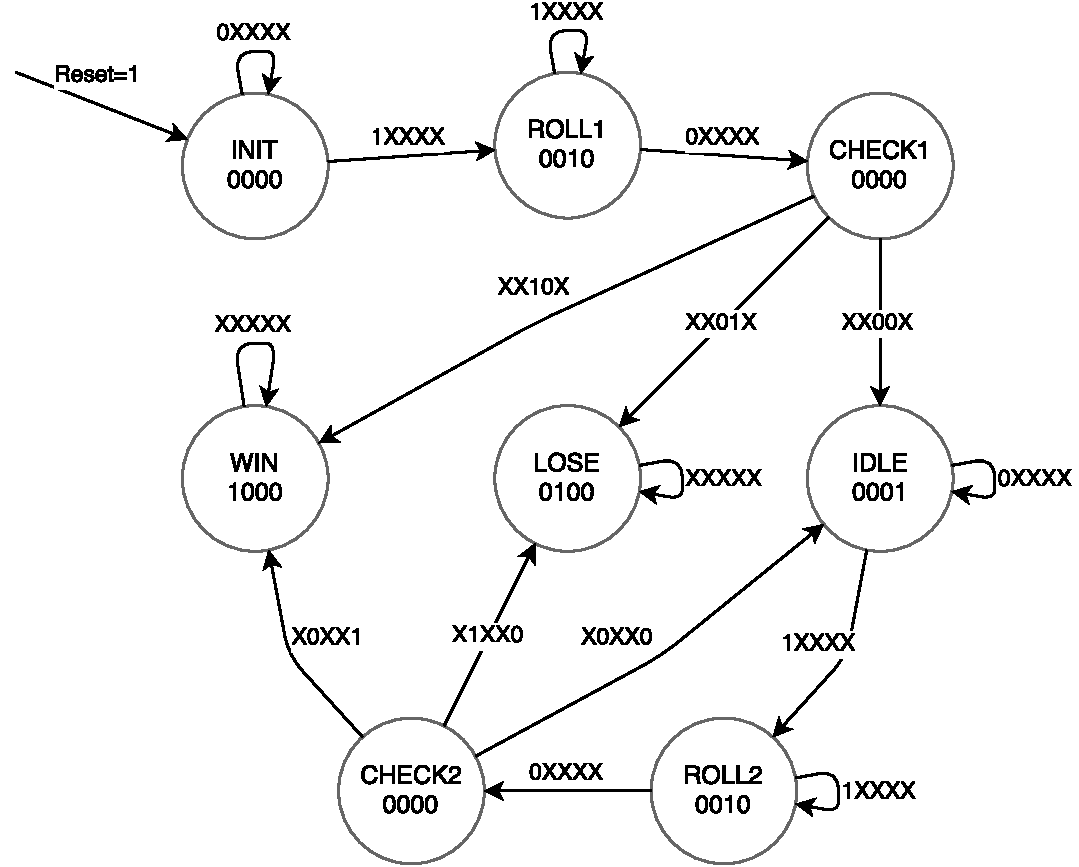
\includegraphics[width=\textwidth]{diceGameDiagram.pdf}
\caption{Przebieg sygnału S2}
\label{diagram:dicegame}
\end{figure}

\subsection{Testbench}

\subsection{Wyniki symulacji}


\section{Model kompletny -- z licznikami i sumatorem}

\subsection{Struktura układu}
\subsection{Testbench}
\subsection{Wyniki symulacji}


\section{Wnioski}

\end{document}






